
\section{Dataset}
This section introduces how we build the whole dataset from raw data. The figure \ref{fig: dataset_overview} shows the process of dataset construction. In the following subsections, we will introduce the operation on each step.

\begin{figure}[htb]
  \centering
  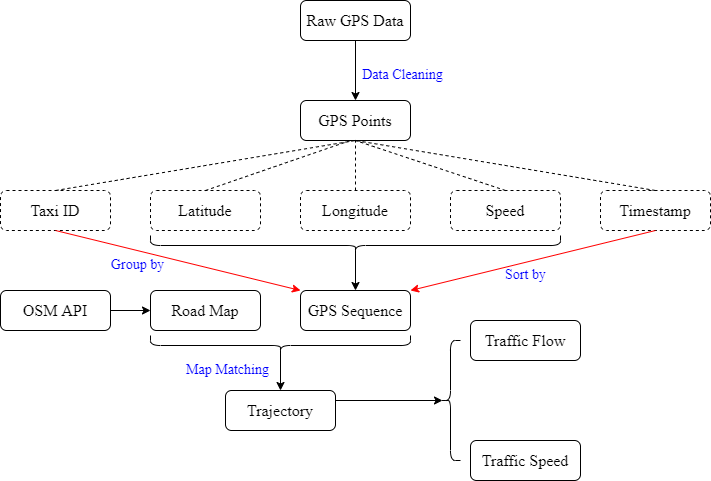
\includegraphics[width=\textwidth]{images/dataset_overview.drawio.png}
  \caption{The flow chart for dataset construction.}
  \label{fig: dataset_overview}
\end{figure}

\subsection{Data Description}
Our data is taken from the records of GPS devices on the taxis in Shenzhen. A brief description is as the following:
\begin{itemize}
    \item \textbf{Region:} Shenzhen
    \item \textbf{Time Range:} June 2020
    \item \textbf{Content:} Taxi GPS records
    \begin{itemize}
      \item License number
      \item Longitude and latitude
      \item Speed
      \item Timestamp
      \item $\cdots$
    \end{itemize}
  \item \textbf{Size:} Over 2,500,000,000 rows
\end{itemize}

A small part of data is shown as an example in figure \ref{fig: raw_data}.
\begin{figure}[htb]
    \centering
    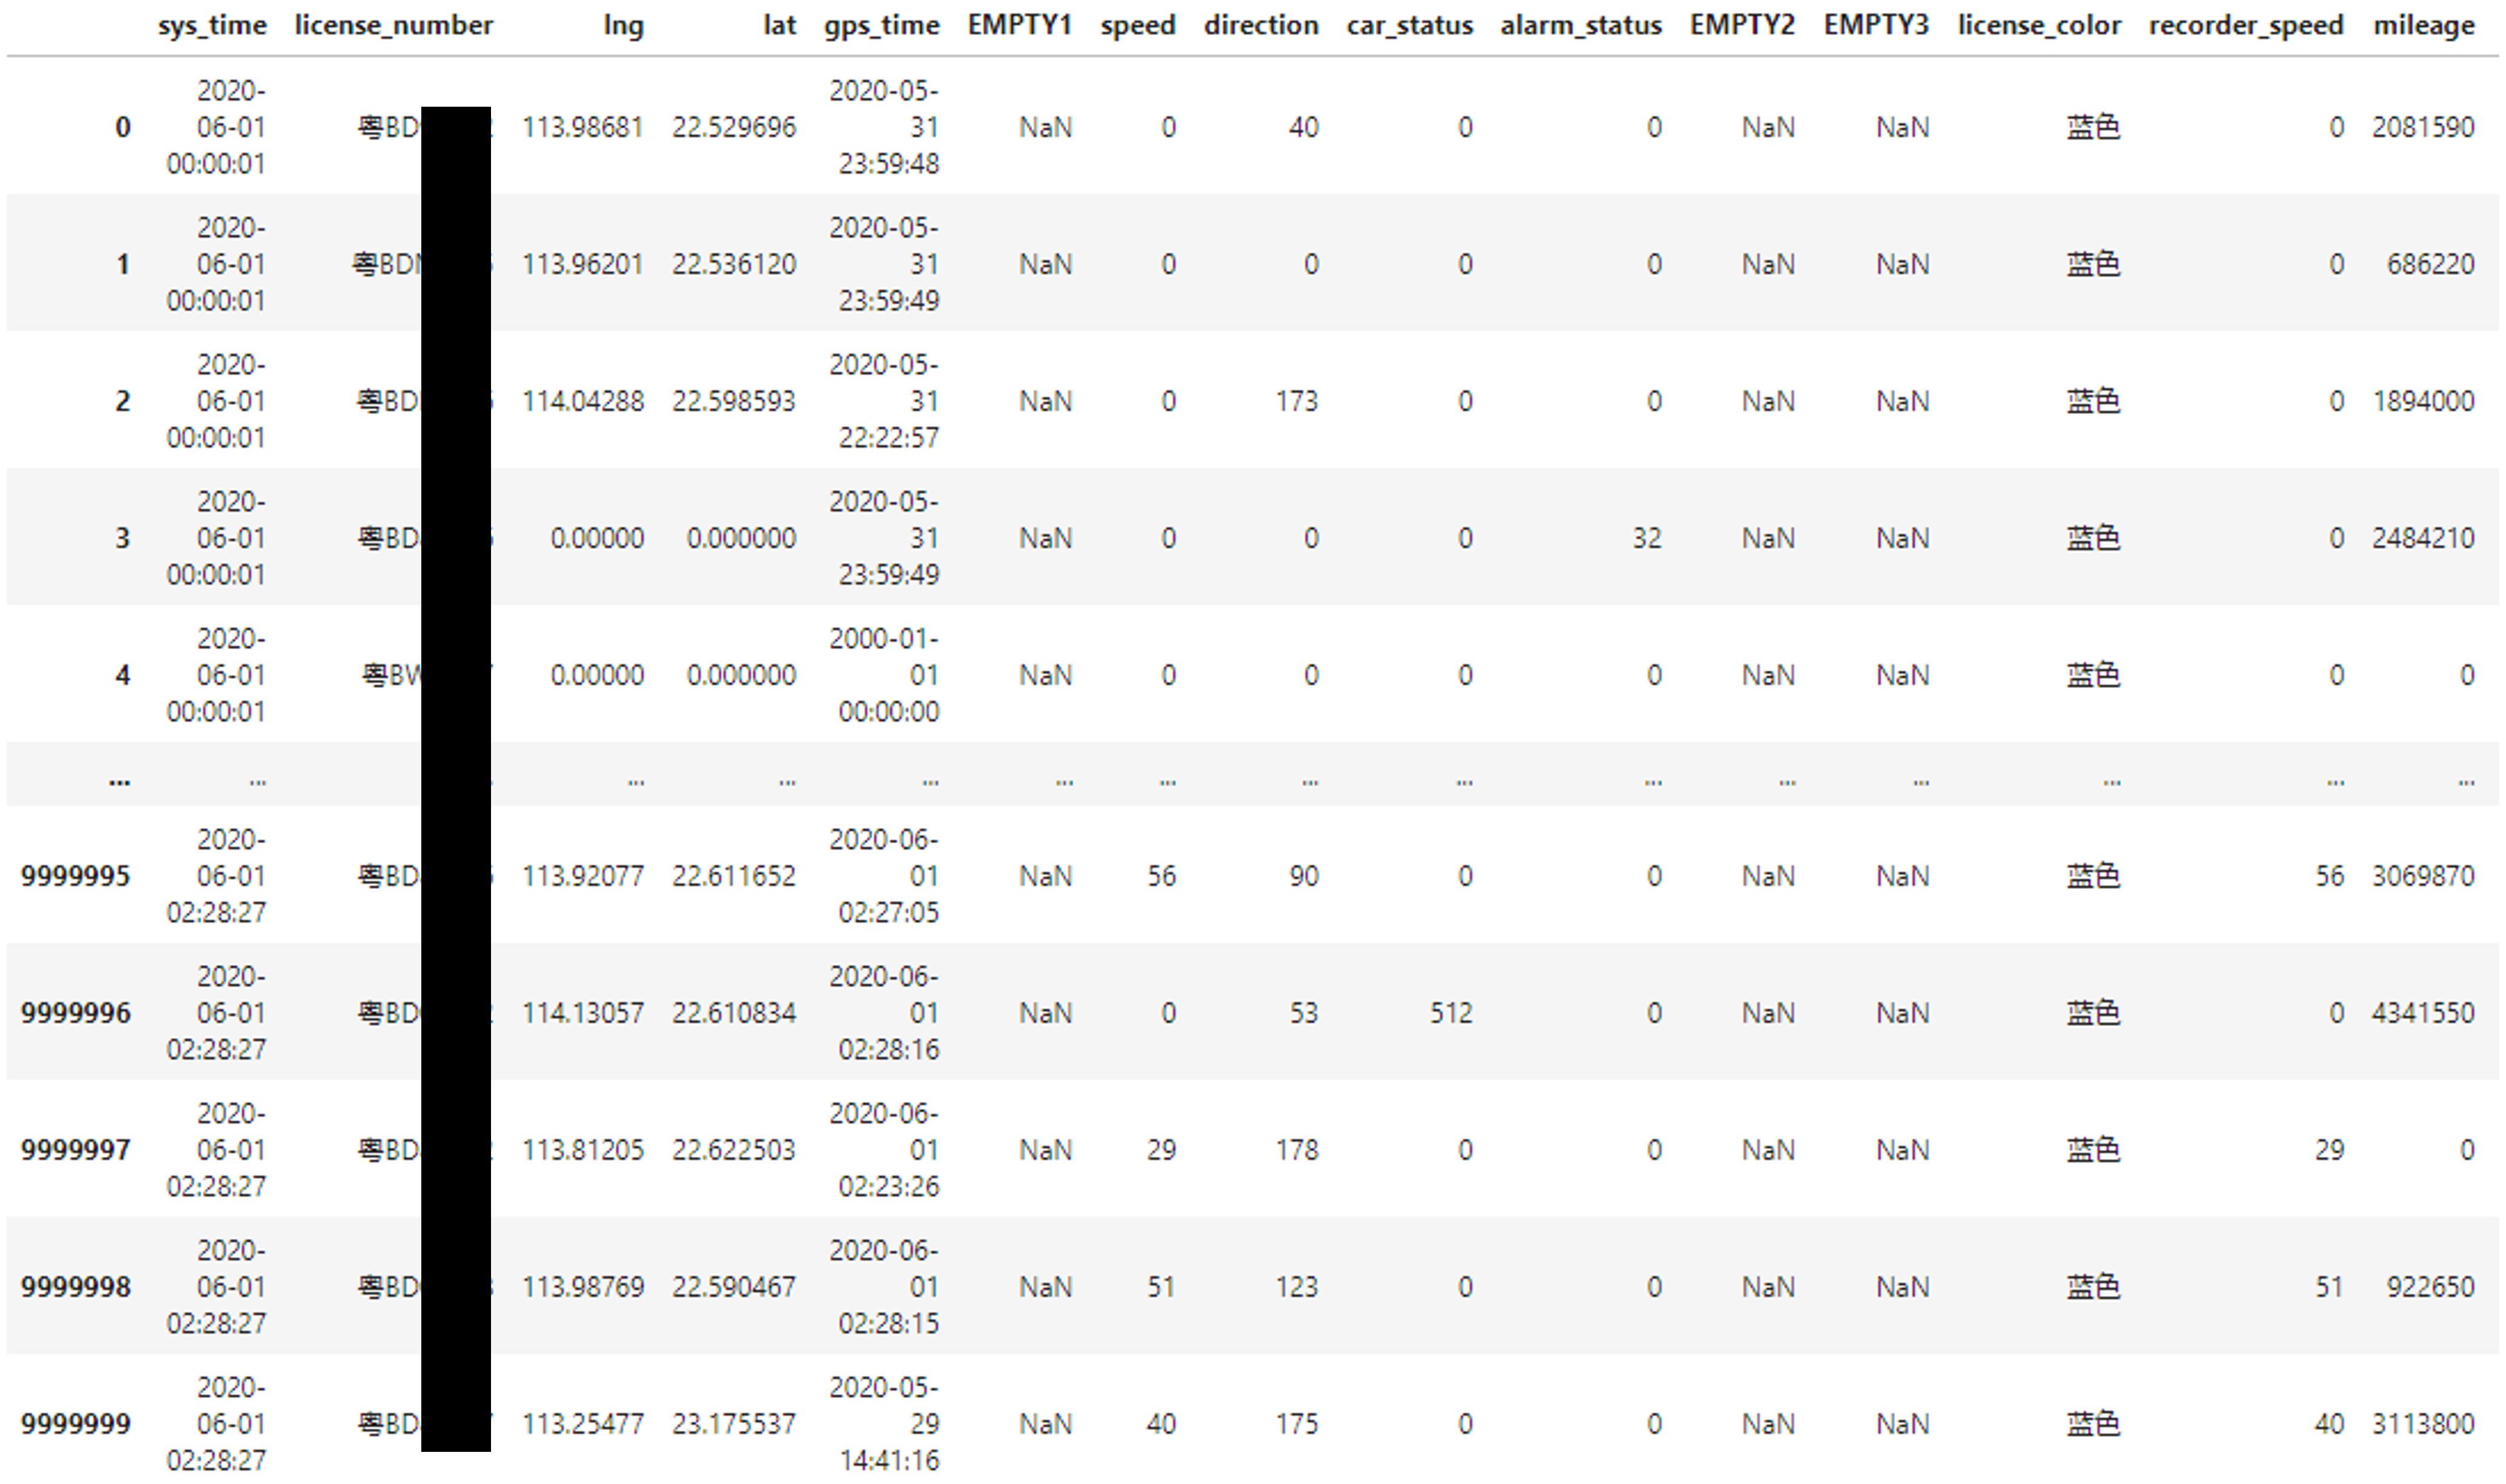
\includegraphics[width=\textwidth]{images/raw_data.png}
    \caption{A glance at Shenzhen taxi GPS raw data.}
    \label{fig: raw_data}
\end{figure}

Unlike the open datasets that can be applied to deep learning models without the need of data cleaning and completion, this raw dataset contains lots of abnormal values, which should be cleaned and re-organized carefully.

\subsection{Data Cleaning}
Data cleaning is the process of detecting and correcting (or removing) corrupt or inaccurate records from a record set, table, or database and refers to identifying incomplete, incorrect, inaccurate or irrelevant parts of the data and then replacing, modifying, or deleting the dirty or coarse data\cite{data_cleaning}. There are many kinds of bad records that should be deleted or modified. To summarize, we categorize them as the following classes.

\begin{enumerate}
  \item \textbf{Duplicate Rows.} A considerable large part of the raw data are duplicate. The reason is when a GPS device is transmitting data to server, it will send several copies in order to avoid packet loss under poor Internet connection. As a result, they are completely same rows, and thus can be removed safely, leaving only the foremost one.
  \item \textbf{Corrupted Timestamp.} This is a sort of abnormal record. Since our time range is June 2020, all the timestamps that not in here should be deleted. In detail, there are two kinds of them: 1) records in May $31^{st}$ or July $1^{st}$. This is caused by the equipments' lack of accuracy. 2) 2000-01-01. And this is caused by data loss, thus, it is filled by a default value.
  \item \textbf{Missing Location.} The latitude and longitude of some records are zero, which is resulted by the data loss during transmission. These dirty values should be deleted.
  \item \textbf{Zero Speed.} Stationary taxis are still transmitting their location information to the server if the GPS device is on, leading to a big portion of zero speed records. They are useless owing to that trajectories are a series of moving locations. Therefore, under normal circumstances, it is better to remove them. However, things are not that happy in our data. There are four kinds of zero speed records relating to the change of location, i.e. latitude and longitude, and they should be treated differently. Details are provided in section 4.5.
  \item \textbf{Irrelevant Attributes.} As shown in figure \ref{fig: raw_data} above, the raw data consists of several columns. The information that have no contribution to trajectories needs to be removed, leaving only latitude, longitude, speed and timestamp.
\end{enumerate}

We take the data of June $1^{st}$ as a case study to give an illustration of our data cleaning procedure and hope to reflect the property of the whole GPS data. In total, there are 97,453,725 rows. Table \ref{data_cleaning_table} gives the deleted percentage and remaining rows after each data cleaning step.

\begin{table}[htb]
  \begin{center}
      \caption{Data cleaning example on June $1^{st}$.}
      \label{data_cleaning_table}
      \begin{tabular}{ccc}
          \toprule

          \textbf{Step} & \textbf{Deleted Percentage} & \textbf{\#Remaining Rows}\\

          \midrule

          Drop duplicate & $51.73\%$ & 47,042,104\\
          Drop abnormal values & $1.19\%$ & 45,874,548\\
          Drop zero speed & $16.84\%$ & 29,458,603\\

          \cmidrule{1-2}

          \textbf{Remaining Percentage} & $30.22\%$ & ~\\

          \bottomrule
      \end{tabular}
  \end{center}
\end{table}

As shown in the table, half of the records are duplicated. Fortunately the total number of records are large enough to endure the data cleaning procedure. For the $17\%$ zero speed records, the following figure \ref{fig: speed_distribution} points out the huge impact of its removal on the distribution of speed.

\begin{figure}[htb]
  \centering
  \caption{Speed distribution before and after cleaning.}
  \label{fig: speed_distribution}
  \begin{subfigure}[t]{0.45\linewidth}
      \centering
      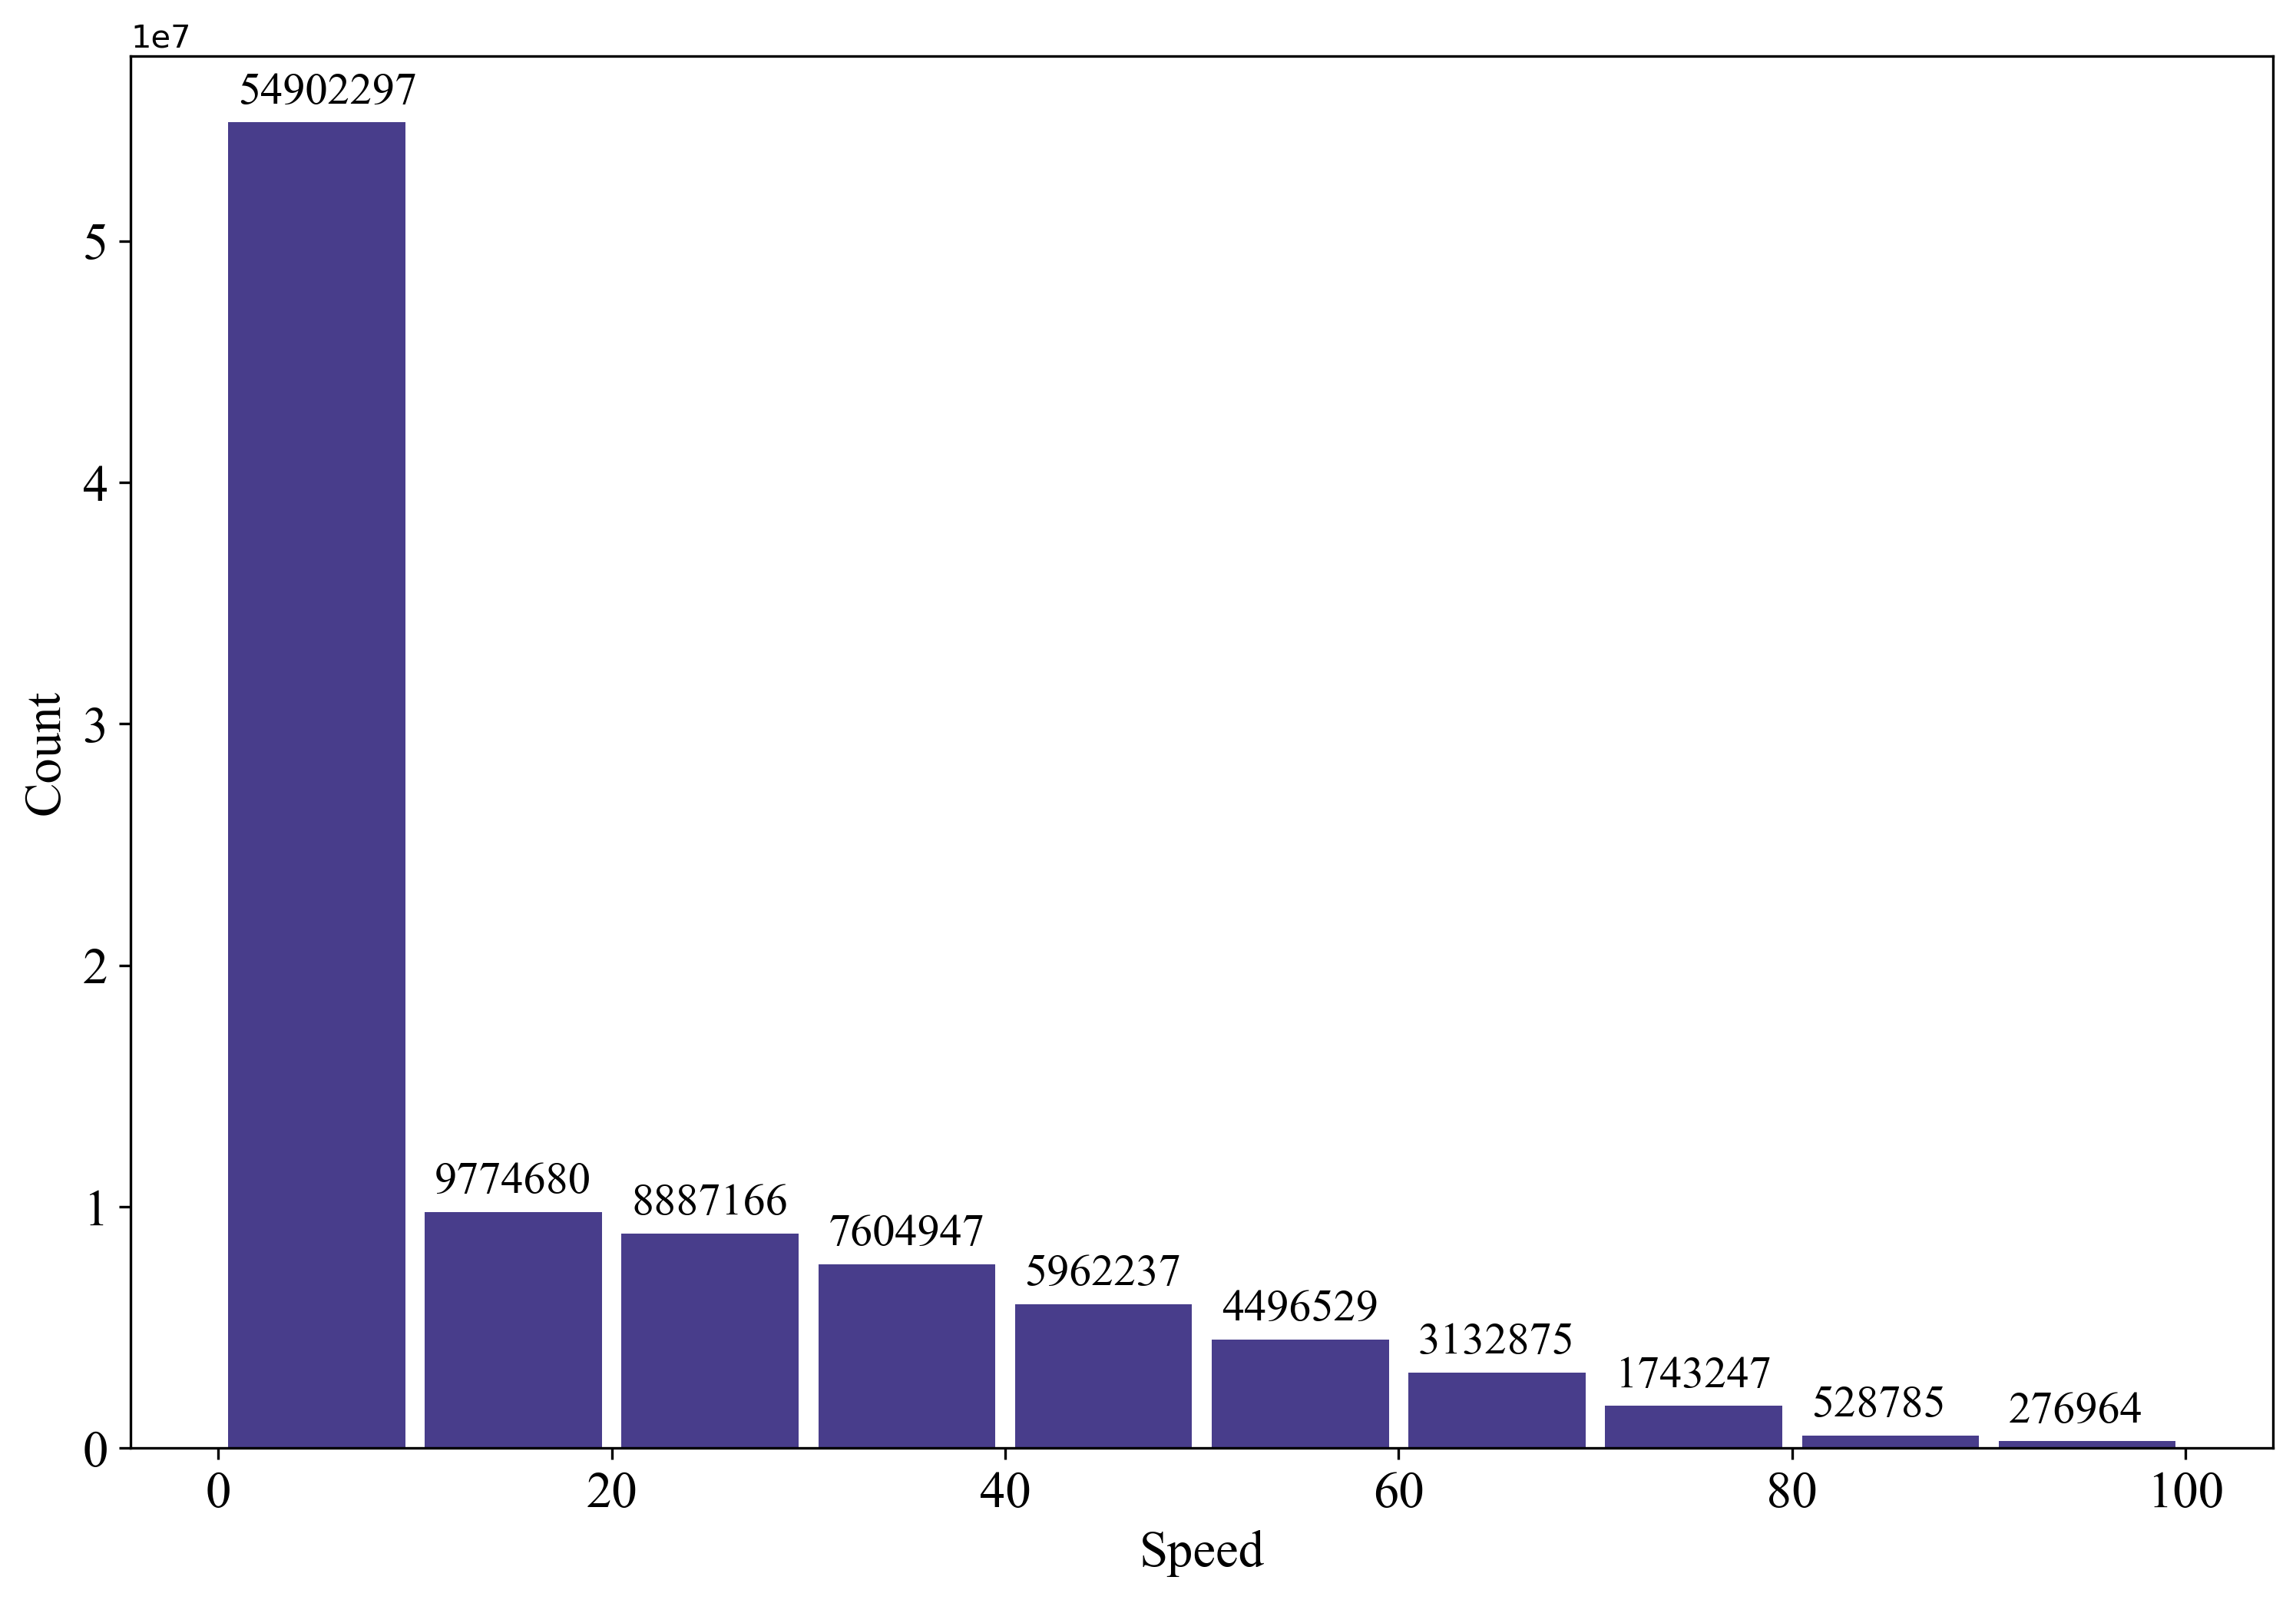
\includegraphics[width=\textwidth]{images/speed_hist_before.png}
      \caption{Before}
      \label{fig: speed_before}
  \end{subfigure}
  \begin{subfigure}[t]{0.45\linewidth}
      \centering
      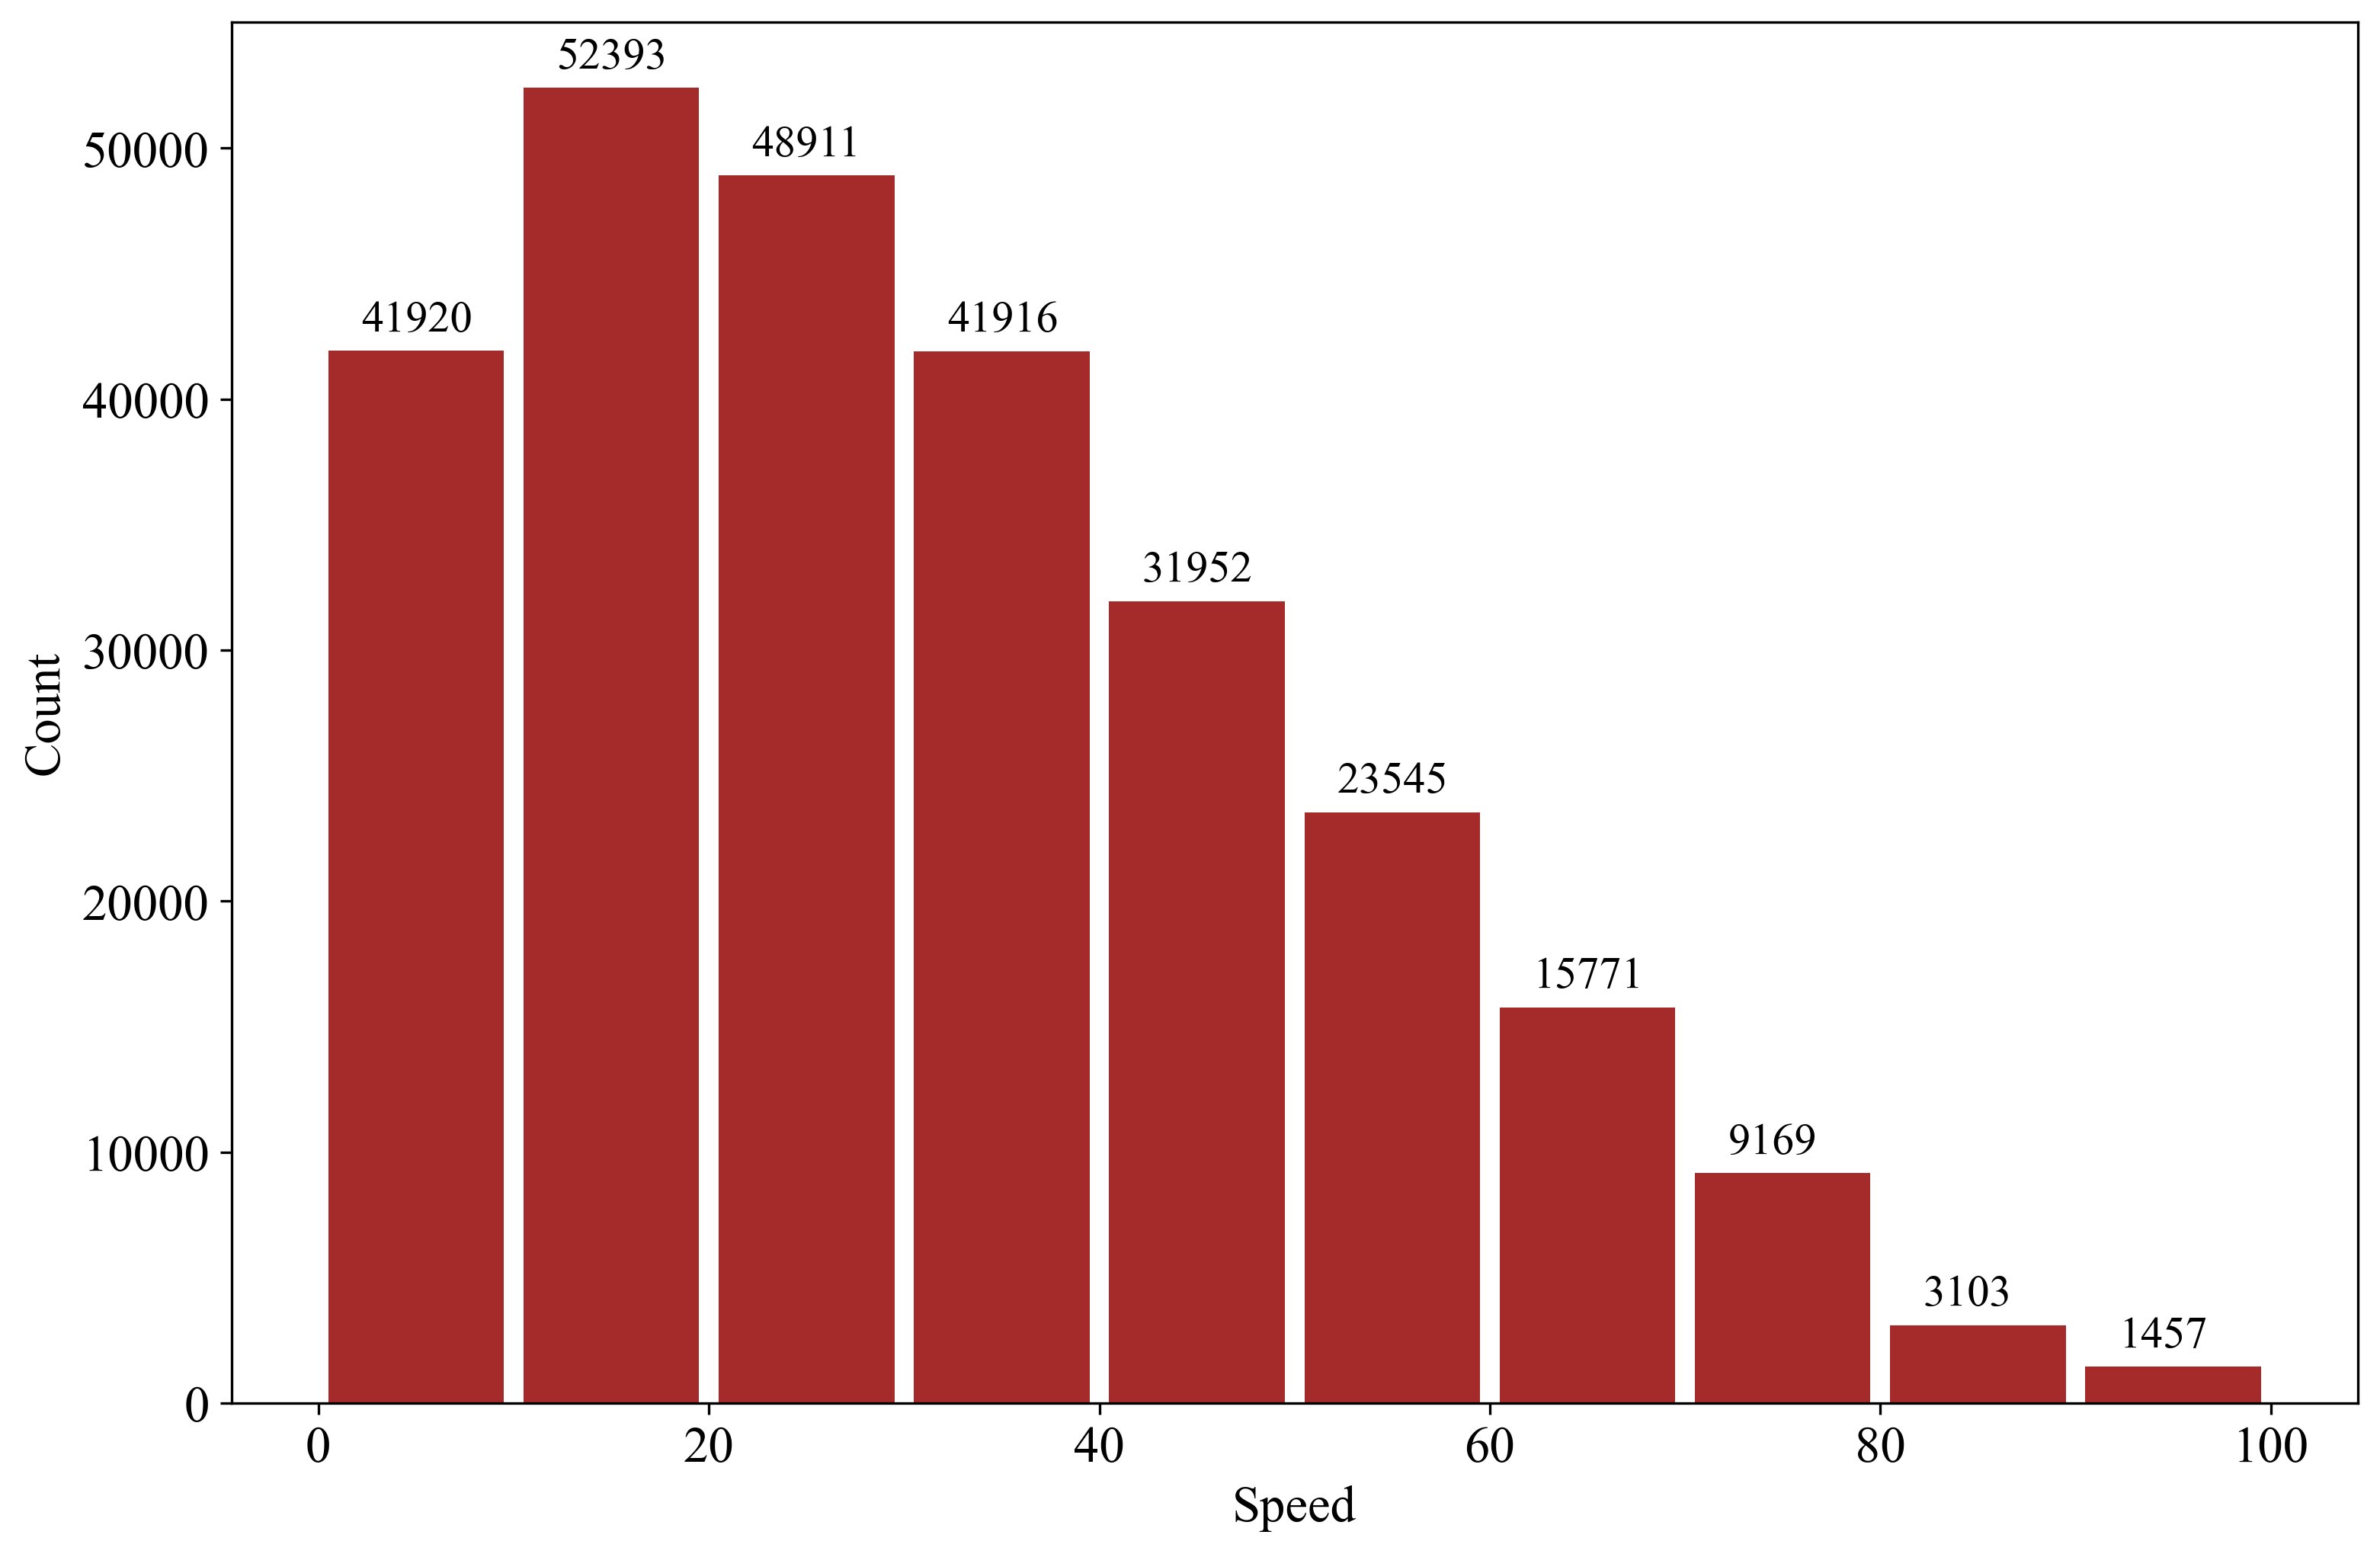
\includegraphics[width=\textwidth]{images/speed_hist_after.png}
      \caption{After}
      \label{fig: speed_after}
  \end{subfigure}
\end{figure}

After data cleaning, we get the GPS point sequences of each car, the next step is to match them to the road network according to their location. But first, we need to draw the GPS points on the map and check if there is any shift with roads, which is related to the coordinate system.

\begin{figure}[htb]
  \centering
  \includegraphics[width=\textwidth]{images/gps_seq.png}
  \caption{Visualization of cleaned GPS points.}
  \label{fig: gps_seq}
\end{figure}

Figure \ref{fig: gps_seq} shows that the GPS points are accurately moving along roads. The coordinate system we use is WGS84 (EPSG: 4326), which is the default for GPS service. Lots of Chinese GPS data is under GCJ-02, an encrypted version of WGS84. The location conversion between them is a complicated task, fortunately there is no need in our dataset.

\subsection{Road Network}
As mentioned in section 2, there are mainly three types of spatial graph that categorized by its vertices, which is grid, sensor or road. For a road network graph, a vertex represents a road and an edge stands for the connectivity between two roads. The formal definition has been given in section 3.3. In short, we need to acquire real road map and construct the graph depending on it.

OpenStreetMap (OSM)\cite{osm} is a collaborative project to create a free editable geographic database of the world. It is easy to download a map and create a road network graph by OSM's official website\footnote{\href{https://www.openstreetmap.org/}{https://www.openstreetmap.org/}} as well as its Python API. Our data covers the taxi tracks over the whole Shenzhen city, however, it is impractical to construct the complete road network due to its huge complexity. As a result, we decide to choose a small region of central business district (CBD) in Futian since it is in one of the most heavy-traffic areas. The red rectangle in figure \ref{fig: gps_seq} encloses the roads we choose, and this is because OSM can only export a rectangular region. % Figure \ref{fig: roadmap} provides a closer look of these roads.
% \begin{figure}[htb]
%   \centering
%   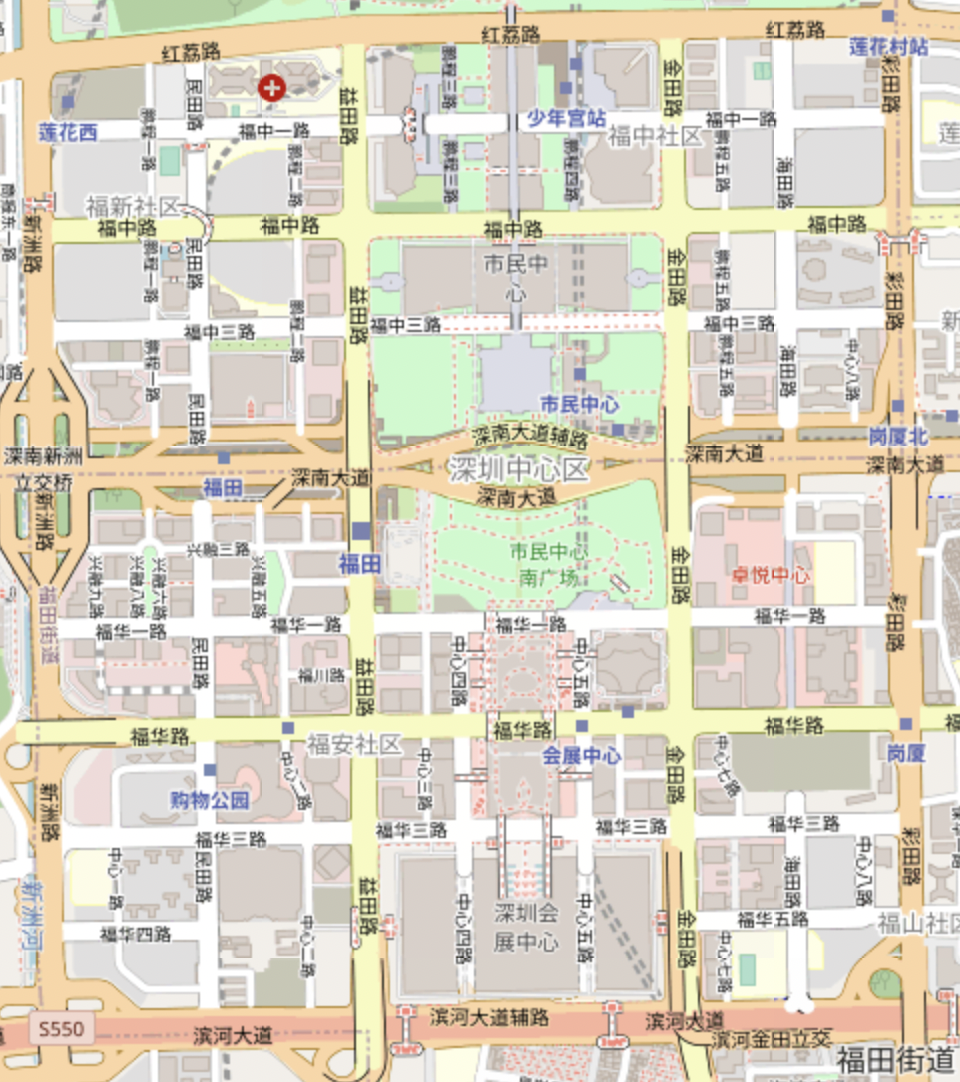
\includegraphics[width=\textwidth]{images/roadmap.png}
%   \caption{The road map for graph construction.}
%   \label{fig: roadmap}
% \end{figure}

\begin{figure}[htb]
  \centering
  \caption{Road network graph before and after simplification.}
  \label{fig: graph}
  \begin{subfigure}[t]{0.45\linewidth}
      \centering
      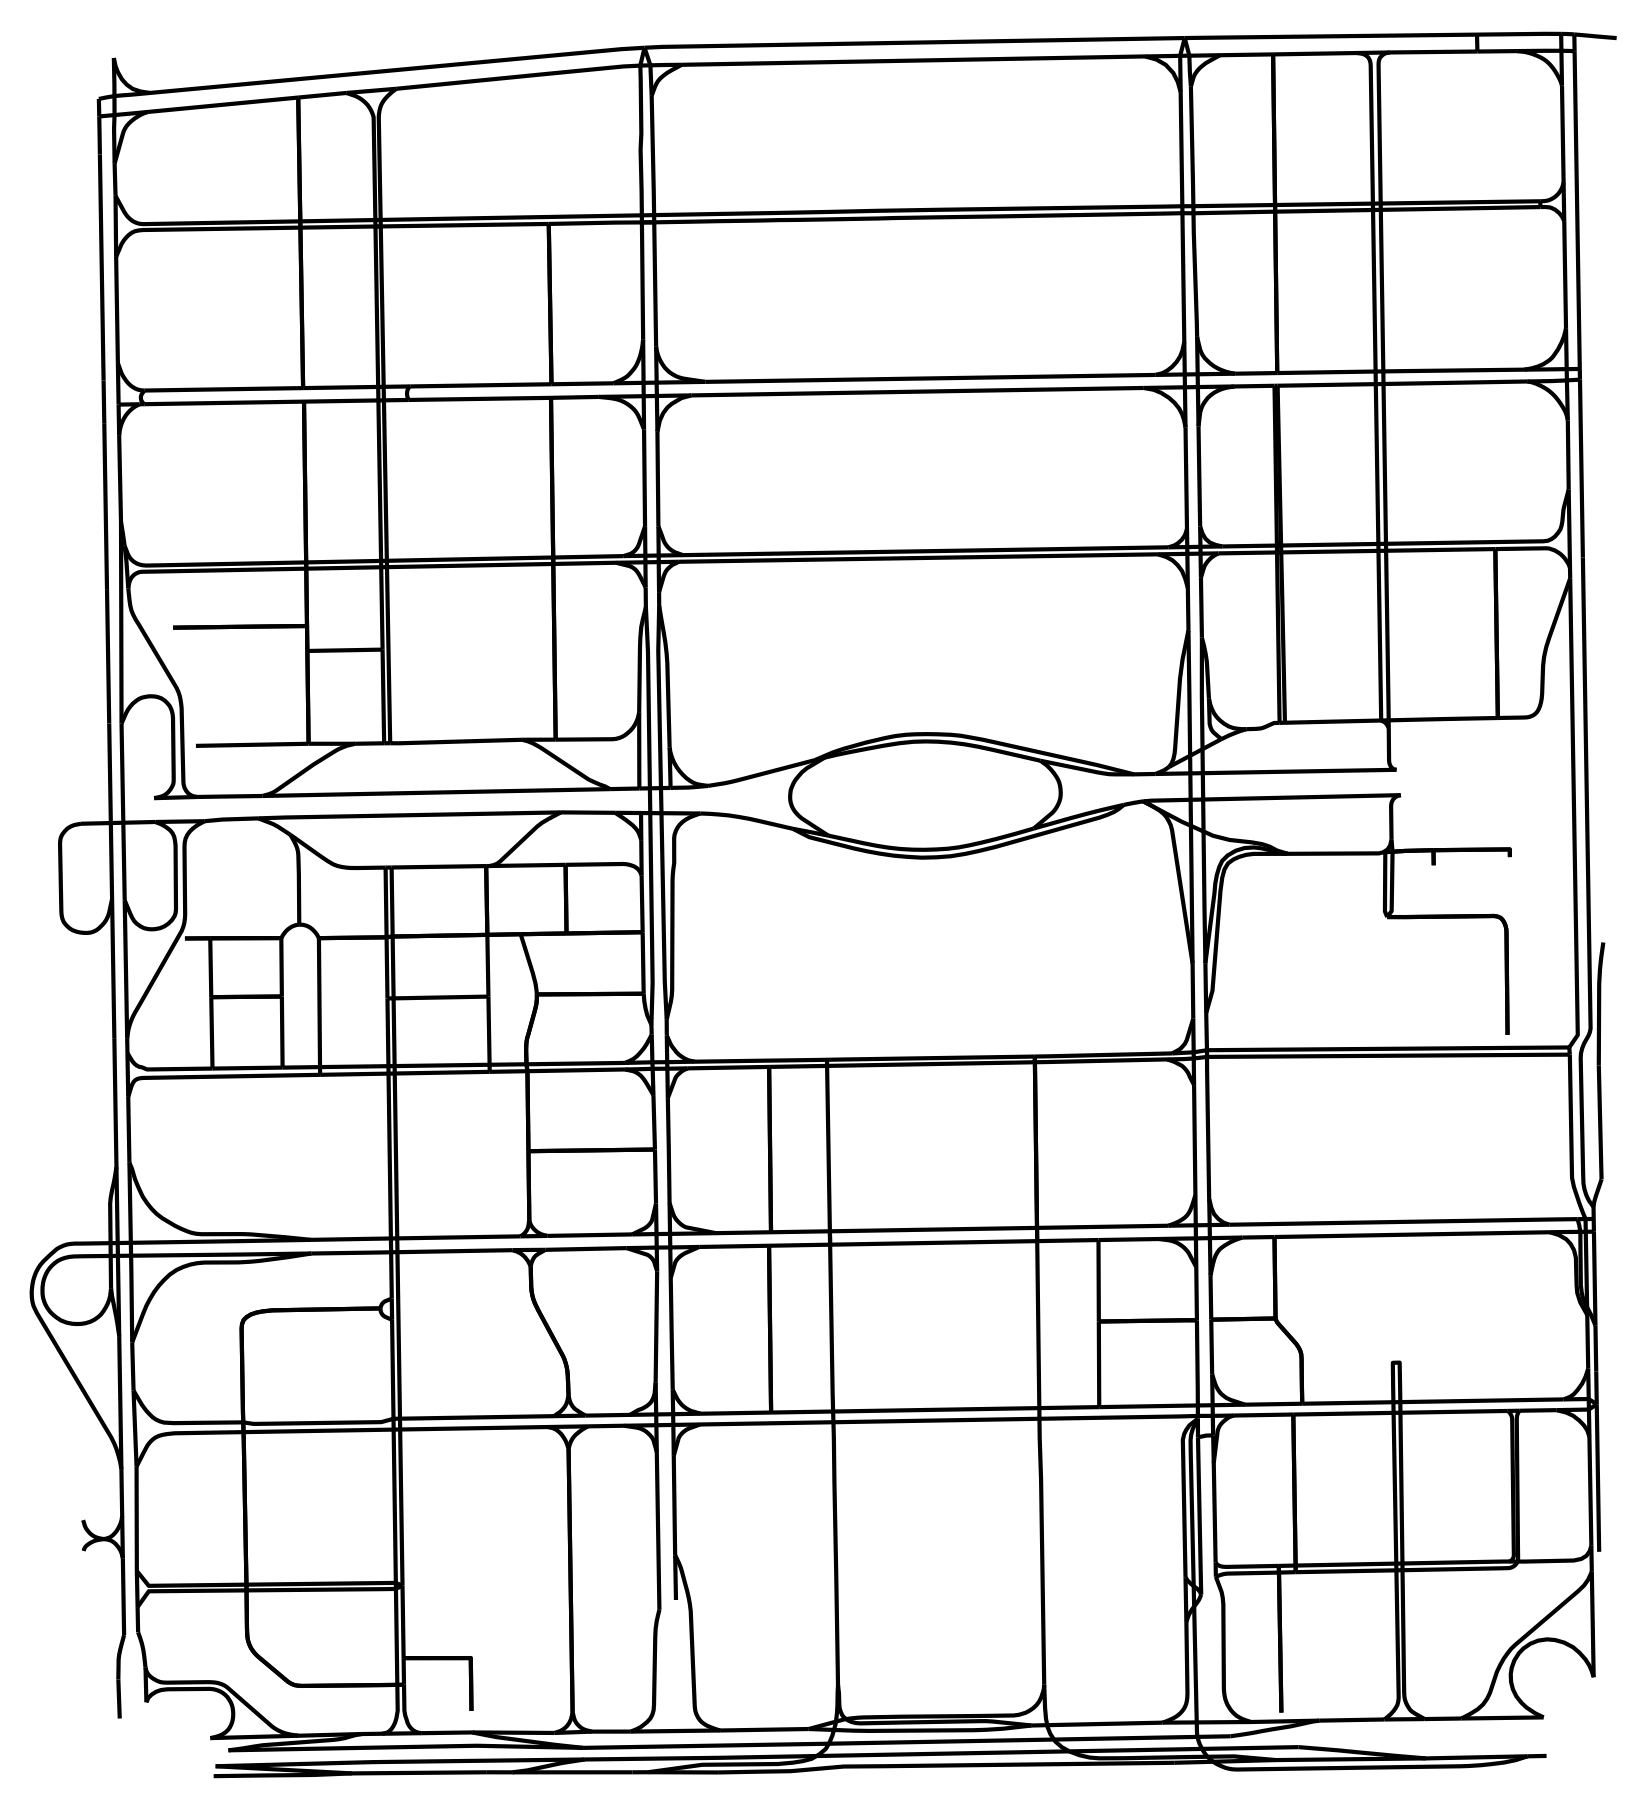
\includegraphics[width=\textwidth]{images/graph_before.png}
      \caption{Before}
      \label{fig: graph_before}
  \end{subfigure}
  \begin{subfigure}[t]{0.45\linewidth}
      \centering
      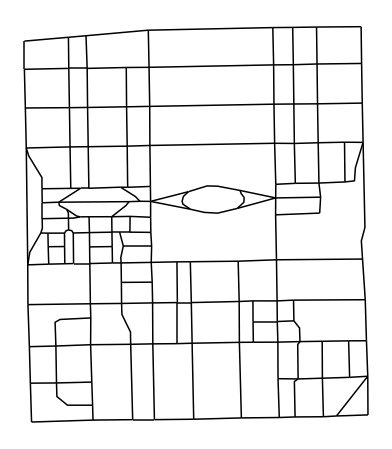
\includegraphics[width=\textwidth]{images/graph_after.png}
      \caption{After}
      \label{fig: graph_after}
  \end{subfigure}
\end{figure}
Having the boundary latitudes and longitudes, we can download the road network as a graph structure via Python. Figure \ref{fig: graph_before} offers the visualization of it. In short, the graph has $906$ roads, $532$ intersections and endpoints. However, this graph still contains plentiful tiny and redundant roads. This is mainly caused by the intersections\cite{graph_simplify}. To be specific, a road will be cut as two roads whenever there is an intersection on it, especially for crossroads. A crossroad is represented by 12 intersection points in the graph, leading to numerous tiny roads that can be merged into main roads. In addition, there are also many other cases that needs to be identified and simplified. To give a better illustration, we summarize them as the following.

\begin{enumerate}
  \item \textbf{Redundant Roads Between Neighboring Intersections.} We have illustrated the reason in the paragraph above. To eliminate them, the simplest way is to merge the intersection points at crossroads.
  \item \textbf{Trailing Roads.} There are some roads not connected to the main road network at both ends. We decide to remove them since they take little effect in traffic.
  \item \textbf{Overpasses.} Overpass is a 3D structure that cannot be reflected in a 2D map. Therefore, the GPS points on overpasses are in a mess when plotting to map, and impossible to be matched on roads. They should be deleted and leaving only the underlying main roads.
  \item \textbf{Two-way Lanes.} Roads are bidirectional, which is faithfully reflected in the graph. However, it will cause a problem that the two lanes of a road do not share the same endpoints. For convenience, we combine them, and manually reverse the road for its bi-directionality.
\end{enumerate}

\begin{figure}[htb]
  \centering
  \caption{Four simplification cases.}
  \label{fig: simplification}
  \begin{subfigure}[t]{0.22\linewidth}
      \centering
      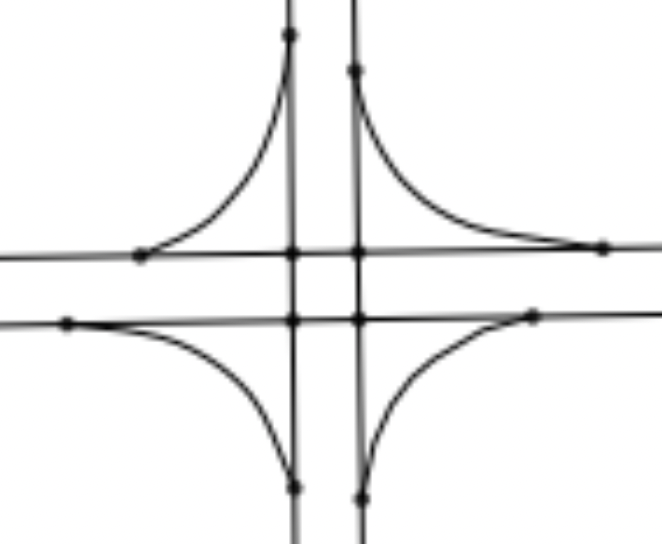
\includegraphics[width=\textwidth]{images/crossroad.png}
      \caption{Redundant Roads}
      \label{fig: redundant_roads}
  \end{subfigure}
  \begin{subfigure}[t]{0.22\linewidth}
      \centering
      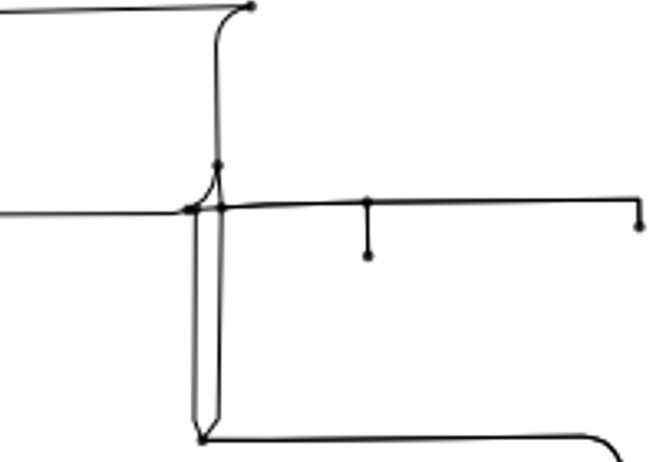
\includegraphics[width=\textwidth]{images/trailing_road.png}
      \caption{Trailing Roads}
      \label{fig: trailing_road}
  \end{subfigure}
  \begin{subfigure}[t]{0.22\linewidth}
    \centering
    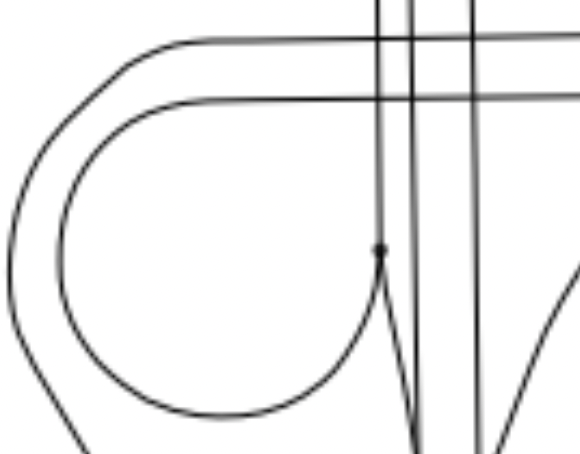
\includegraphics[width=\textwidth]{images/overpass.png}
    \caption{Overpass}
    \label{fig: overpass}
  \end{subfigure}
  \begin{subfigure}[t]{0.22\linewidth}
    \centering
    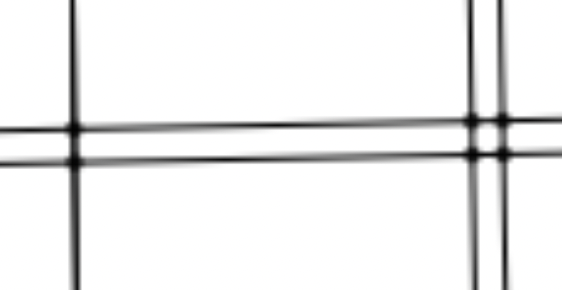
\includegraphics[width=\textwidth]{images/two-way.png}
    \caption{Two-way Lanes}
    \label{fig: two-way}
  \end{subfigure}
\end{figure}

A visualization of these four cases is provided by figure \ref{fig: simplification}. To handle them, we use QGIS\footnote{\href{https://qgis.org/en/site/}{https://qgis.org/en/site/}} as a tool to redraw the graph by ourselves. QGIS functions as geographic information system (GIS) software, allowing users to analyze and edit spatial information, in addition to composing and exporting graphical maps. Figure \ref{fig: graph_after} shows the road network graph $\mathcal G$ after simplification where the four cases are eliminated thoroughly. As a result, it has $n_r=492$ roads. 

\subsection{Map Matching}
Map matching\cite{mm} is a procedure to match a location, in this paper, a \textit{(latitude, longitude)} pair, on a specific road to determine where the vehicle is travelling on. A variety of map matching algorithms have been proposed by researchers around the world in recent years, such as Hidden Markov Map Matching\cite{HMMM}, ST-Matching\cite{stmm} and Fast Map Matching\cite{fmm}. We tried several map matching functions and eventually choose Fast Map Matching (FMM) because of its fastest speed and open-source library.

\begin{table}[htb]
  \begin{center}
      \caption{FMM tuned parameters.}
      \label{fmm_table}
      \begin{tabular}{cll}
          \toprule

          \textbf{Parameter} & \textbf{Description} & \textbf{Value}\\

          \midrule

          $\delta$ & Upper bound & $0.03$\\
          $k$ & Number of candidates & $8$\\
          $r$ & Search radius & $0.003$\\
          $e$ & GPS error & $0.0005$\\

          \bottomrule
      \end{tabular}
  \end{center}
\end{table}

Table \ref{fmm_table} provides the tuned parameters we apply on map matching, and the description of them are taken from FMM's official document. As a result, we achieved $100\%$ matched percentage. After FMM, we get the matched trajectories. To limit their length, we split a trajectory if GPS reading is off for over 10 minutes. Finally, the trajectory set $\mathcal{T}$ is generated.

\subsection{Data Interpolation}
In the data cleaning stage, we removed $70\%$ rows in the June $1^{st}$ example. Although most of them are duplicated, there are still some records that can be taken use of, which is related to the four cases of zero speed records that we mentioned in section 4.2. In addition, due to the low and unstable sampling rate of the GPS devices, \textbf{discontinuities} are prevalent in the trajectories. Here we give a detailed explanation of their causes and countermeasures.

\vspace{\baselineskip}

\textbf{The four zero speed cases.} Note that these cases are for consecutive records in the raw data.
\begin{enumerate}
  \item \textit{Location: unchanged, Timestamp: unchanged.} This is duplication, which we have already removed at first.
  \item \textit{Location: unchanged, Timestamp: changing.} This case indicates that the vehicle is not moving, exactly what we want to delete.
  \item \textit{Location: changing, Timestamp: unchanged.} Device abnormality, because one vehicle cannot drive on different roads at the same time. They should be deleted.
  \item \textit{Location: changing, Timestamp: changing.} The vehicle is moving, however, its speed becomes zero. This is the part we try to interpolate. The method is, we use latitude, longitude and timestamp to calculate the real distance and time duration of the two adjacent locations, and use a simple division to compute the speed.
\end{enumerate}

\vspace{\baselineskip}

\textbf{Discontinuities in trajectories.} We illustrate this problem with an example in figure \ref{fig: traj_interpolate}. The three red points are from raw data, after map matching, we get a trajectory $[r_1, r_3, r_4]$. However, owing to the topology of the road network graph, the vehicle must pass $r_2$ and $r_3$. For some reason like the low recording frequency of the GPS device, the points on $r_2$ and $r_3$ are not recorded. To deal with it, we take use of an FMM's built-in function that is able to interpolate the missing points and output the trajectory $[r_1, r_2, r_3, r_4, r_5]$. Trajectory interpolation is \textbf{essential} because the dataset will have a very, very bad performance on traffic prediction models without it.

\begin{figure}[htb]
  \centering
  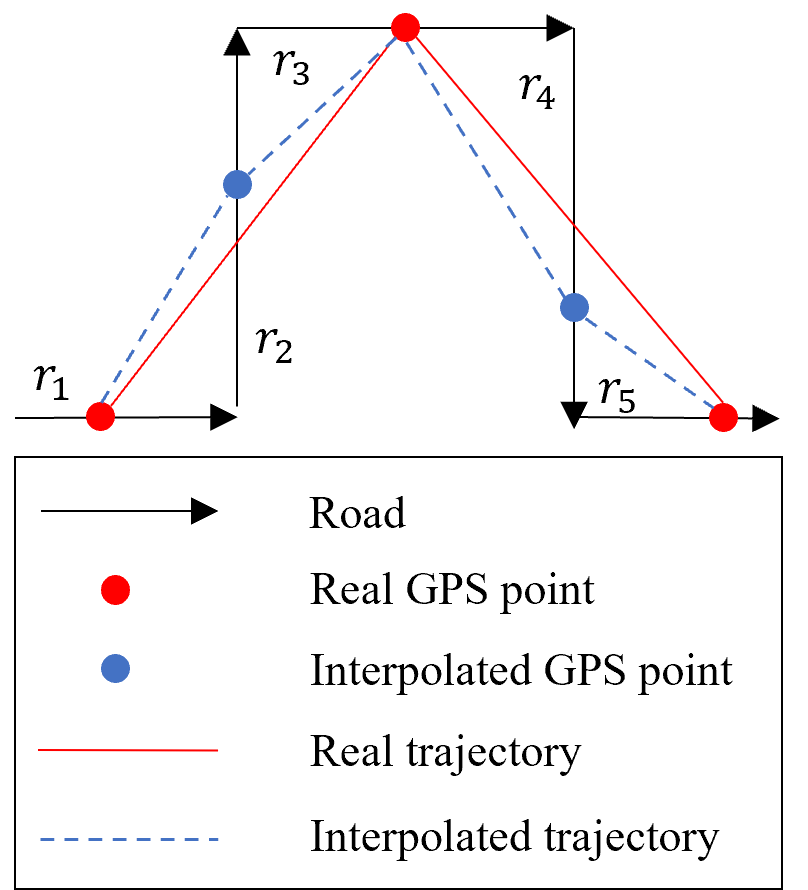
\includegraphics[width=0.5\textwidth]{images/traj_interpolate.png}
  \caption{Interpolation for the discontinuity in a trajectory.}
  \label{fig: traj_interpolate}
\end{figure}

\subsection{Road Traffic States}
The last step is to count the traffic states of each road. Having a trajectory as a $(r, s, ts)$ sequence, the traffic flow of $r$ at the corresponding time interval will be increased. \textbf{And the length of each time interval is 5 minutes in our work.} For instance, if there is a tuple $(r_1, 40, 12:03)$, then the flow of $r_1$ at interval $12:00 - 12:05$ is increased by $1$. The traffic speed of $r_1$ is the sum of all related tuples' speed divided by its flow. If no vehicle pass by in a time interval, we assume its traffic speed is the average of all other time intervals. As a result, we collect the traffic flow and speed of all roads into traffic state matrix $X$, and both of $X_{flow}$ and $X_{speed}$ have size $(n_r, n_t)$.
